\chapter{Introdução}
\label{cap:introducao}

\section{Problema e contexto}

A abordagem convencional no desenvolvimento de sistemas corporativos, na qual toda a lógica de negócio, persistência e apresentação são encapsuladas em uma única aplicação (e um único executável), é a mais natural para construção desse tipo de sistema. Essa arquitetura, conhecida comumente como monólito, tem alcançado sucesso devido à sua simplicidade no desenvolvimento, testes, implantação e monitoramento, entre outros fatores. No entanto, com a popularização da computação em nuvem, a crescente demanda de mudanças cada vez mais frequentes e o crescimento das equipes de tecnologia da informação em grandes organizações, essa arquitetura é confrontada com desafios significativos. Inicialmente, destaca-se o acoplamento nos ciclos de mudanças, onde qualquer alteração em uma pequena parte requer a compilação e implantação de todo sistema. Além disso, há dificuldade em escalar horizontalmente apenas funcionalidades específicas que estão sendo mais demandas e existe complexidade na utilização de diferentes linguagens de programação em diversas áreas de um sistema \cite{microservices}. Por esses motivos, a adoção da \acrfull{ams} cresceu de forma exponencial nos últimos anos, com 77\% dos profissionais afirmando que suas organizações utilizam esse estilo arquitetural \cite{microserviceAdoption}.

Por outro lado, \english{\acrfull{ddd}} é uma abordagem para o desenvolvimento de software, na qual os elementos de software como pacotes, classes, interfaces, métodos e nomes de variáveis devem corresponder aos conceitos do domínio de negócio \cite{dddFowler}. Adicionalmente, o \acrshort{ddd} se configura como uma estratégia para harmonizar especialistas de negócios, desenvolvedores e projetistas, promovendo uma otimização nas interações ao reduzir o mapeamento entre termos de negócio e termos técnicos.

Em agosto de 2008, um grande incidente interrompeu as operações da \emph{Netflix}, empresa que nesse período alugava DVDs através de seu site na \english{web}. Uma corrupção no banco de dados impediu que a companhia pudesse realizar envios por três dias. A partir desse momento, os engenheiros perceberam que necessitavam reduzir pontos únicos de falha, tais como grandes bases de dados relacionais armazenadas em somente um \english{data center}. Em vez disso, optaram por adotar sistemas distribuídos na nuvem, escalonados horizontalmente, para garantir maior confiabilidade e minimizar o impacto das falhas \cite{netflixMigration}.

Essa transição resultou em vários benefícios para a \emph{Netflix}, destacando-se a conquista de uma disponibilidade de 'quatro noves' (99,99\%) e significativa redução de custos. Além disso, a \short{ams} permitiu que diferentes aplicações utilizassem diferentes tecnologias, facilitando contratações e extraindo o melhor de cada opção. Assim, em 2016 (8 anos após a migração) a empresa tinha 8 vezes mais assinantes, muito mais ativos, com o número de visualizações crescendo em três ordens de grandeza nesse período \cite{netflixMigration}.

A \acrshort{ams} e \acrshort{ddd} podem ser combinados no \english{design} e desenvolvimento de sistemas. De um lado, microsserviços possibilitam escalabilidade independente, implantação desacoplada e utilização de múltiplas tecnologias para determinados casos de uso. Por outro lado, \acrshort{ddd} fornece uma abordagem para modelagem do domínio de negócio, diversos padrões para resolver problemas de modelagem recorrentes e facilidade de entendimento e manutenção de código. Além disso, \acrshort{ddd} é uma excelente estratégia para definição de limites entre microsserviços. Ao modelar os serviços com base em \english{\acrfull{bc}}s coesos, é possível o desenvolvimento de novas funcionalidades mais rapidamente e também se torna mais simples a recombinação de microsserviços para fornecer novas funcionalidades aos usuários \cite{buildingMicroservices}.

\section{Justificativa}

Recentemente, observou-se um notável crescimento em popularidade e adoção da \acrshort{ams} e da abordagem \acrshort{ddd} no desenvolvimento de sistemas corporativos. Porém, essas tecnologias são utilizadas de maneira equivocada em muitas implementações devido à falta de compreensão das suas vantagens e desvantagens, entre outros fatores. Por exemplo, a equipe de desenvolvimento do \emph{Amazon Prime Video} recentemente anunciou uma migração de um serviço de monitoramento de vídeo, que foi inicialmente desenvolvido com microsserviços, para uma arquitetura monolítica com objetivo de aumentar a escalabilidade e reduzir custos \cite{amazonBackMigration}.

Paralelamente a isso, é possível identificar uma carência de estudos de caso realistas envolvendo a utilização simultânea da \acrshort{ams} e \acrshort{ddd}, especialmente no cenário nacional.  Enquanto algumas publicações concentram-se exclusivamente em um desses conceitos e outras apresentam exemplos simplificados, proporcionando uma compreensão limitada de como essas duas técnicas podem ser efetivamente empregadas em conjunto. 

Nesse contexto, este trabalho visa preencher essa lacuna ao oferecer uma contribuição significativa para a compreensão da aplicação integrada dessas estratégias no desenvolvimento de sistemas. Por meio de um estudo de caso realista, busca-se não apenas enriquecer o conhecimento acadêmico, mas também fornecer uma base sólida para a implementação prática dessas tecnologias em diversos setores da indústria.

\section{Objetivos}

\subsection{Objetivo Geral}
O objetivo geral deste trabalho de conclusão de curso é apresentar um estudo de caso realista integrando a \acrshort{ams} e \acrshort{ddd}, visando demonstrar como essas tecnologias podem ser utilizadas para aumentar a escalabilidade, desempenho e resiliência de sistemas complexos.


\subsection{Objetivos Específicos}
\begin{itemize}
\item Apresentar uma estratégia para transformar requisitos funcionais em um \english{design} com \acrshort{ams} e \acrshort{ddd}.
\item Prover informações relevantes para definição dos estilo de comunicação adequado entre microsserviços.
\item Demonstrar desempenho e escalabilidade do sistema desenvolvido através de testes de carga.
\end{itemize}

\section{Metodologia}
Pode-se observar na \autoref{fig:metodo_recurso} as etapas de execução dessa pesquisa. Inicialmente, o escopo é definido e o primeiro capítulo é elaborado. Em seguida, a fundamentação teórica com os conceitos-chave é construída. Posteriormente, se realiza um mapeamento da literatura buscando trabalhos similares. Por último, um estudo de caso realista com a utilização de microsserviços e diversos conceitos do \acrshort{ddd} é desenvolvido e um relatório é produzido. Por fim, é escrita a conclusão do trabalho.

% \vfill

\begin{figure}[h!]
    \centering
    \caption{Etapas de desenvolvimento da pesquisa}
    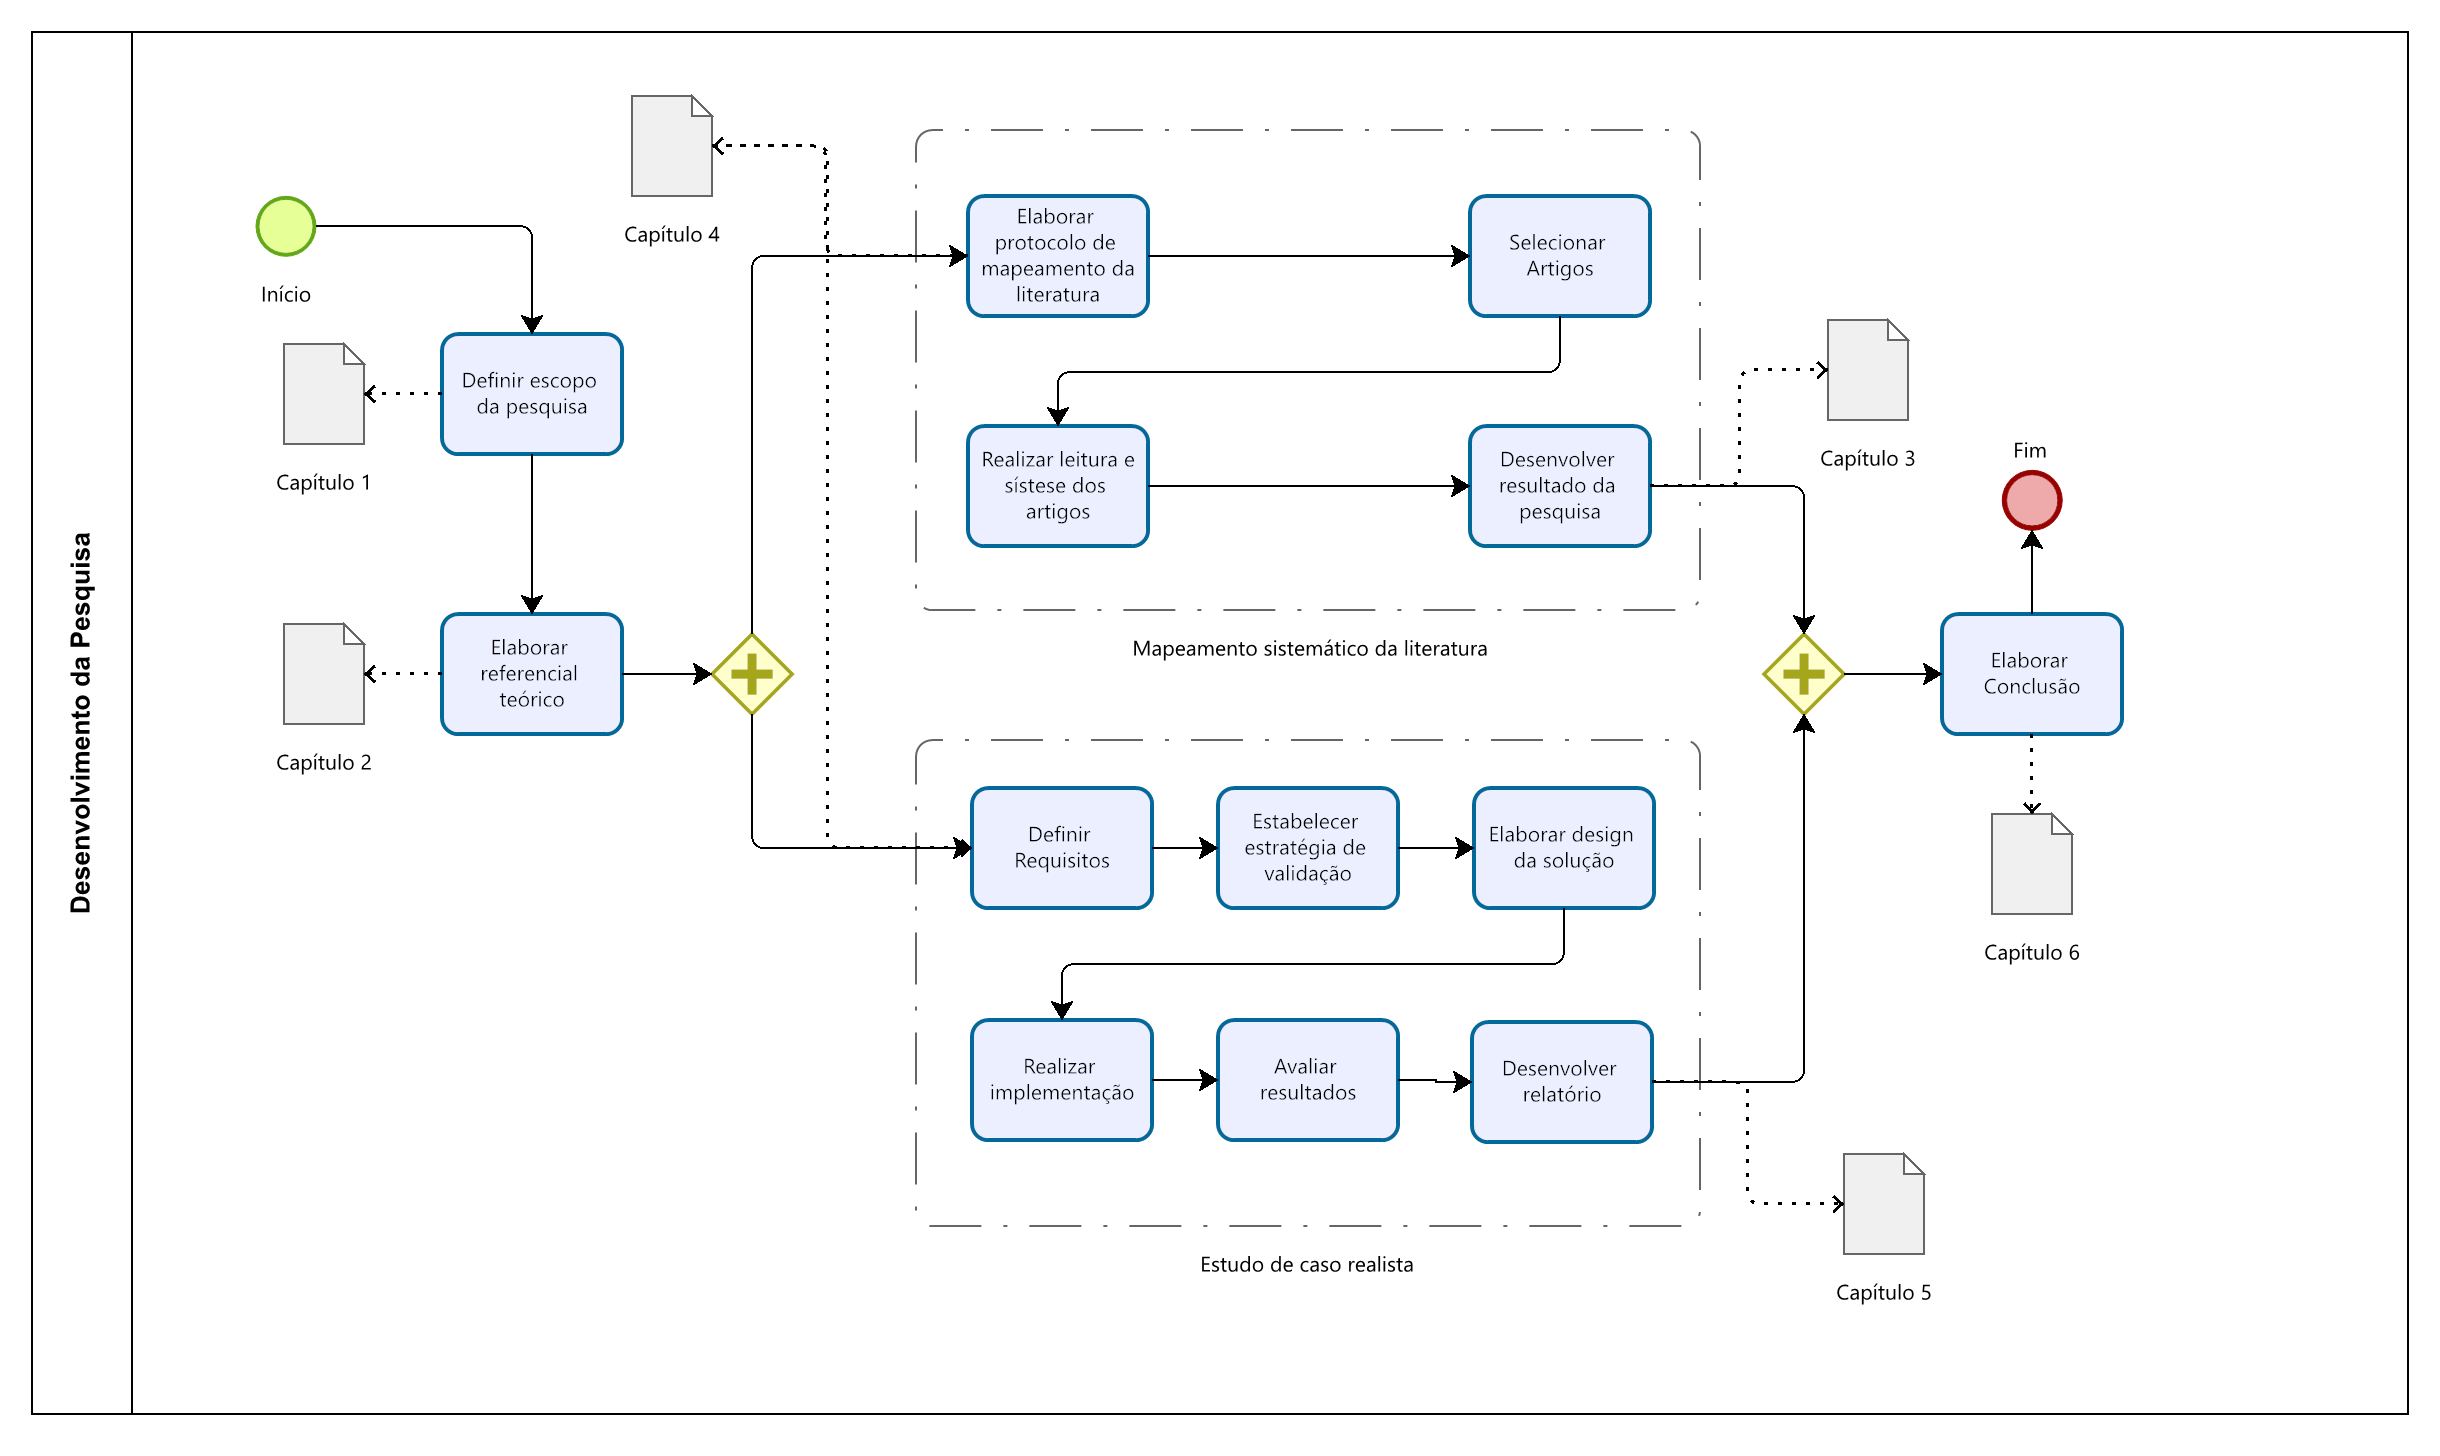
\includegraphics[width=0.9\textwidth]{media/bpmn_metodo_recurso.png}
    \legend{Fonte: o autor}
    \label{fig:metodo_recurso}
\end{figure}



\section{Estrutura do Trabalho}

Este trabalho está dividido em sete capítulos.  O \autoref{cap:introducao} expõe o contexto do estudo, as justificativas desta pesquisa e os objetivos a serem atingidos. O \autoref{cap:fundamentacao} apresenta conceitos de \acrshort{ddd}, \acrshort{ams} e afins. O \autoref{cap:trabalhos} expõe o protocolo e o resultado do mapeamento da literatura sobre a utilização combinada das estratégias mencionadas. Da mesma forma, o \autoref{cap:estudo_caso1} descreve os requisitos, métodos e organização do estudo de caso. Em seguida, o \autoref{cap:estudo_caso2} apresenta o estudo de caso desenvolvido, incluindo o \english{design} do sistema, trechos de código chave da implementação. Posteriormente, o \autoref{cap:resultados} apresenta os resultados obtidos com a execução dos testes de carga e uma discussão sobre os desafios e benefícios da utilização de \acrshort{ddd} e \acrshort{ams}. Por fim, o \autoref{cap:conclusão} apresenta as conclusões obtidas com o desenvolvimento deste trabalho.